%%%%% Section 5. Demonstration with real data %%%%%
\section{Facet-Induced Connotation Spaces from Real Data}
\label{sec:demonstration}

Section~\ref{sec:mathematics} took the ideal content space as given. Here we
take it as data. Modern general-purpose encoders---CLIP, CLAP, and the
like---aim at the same ideal: trained on large corpora, for no single task, they
turn likeness into closeness. So their embeddings serve as content data. This
section builds two libraries, one from sound and one from sight, and reads the
connotation space each one gives.

\begin{figure}[p]
    \centering
    \begin{subfigure}[t]{0.48\linewidth}
        \centering
        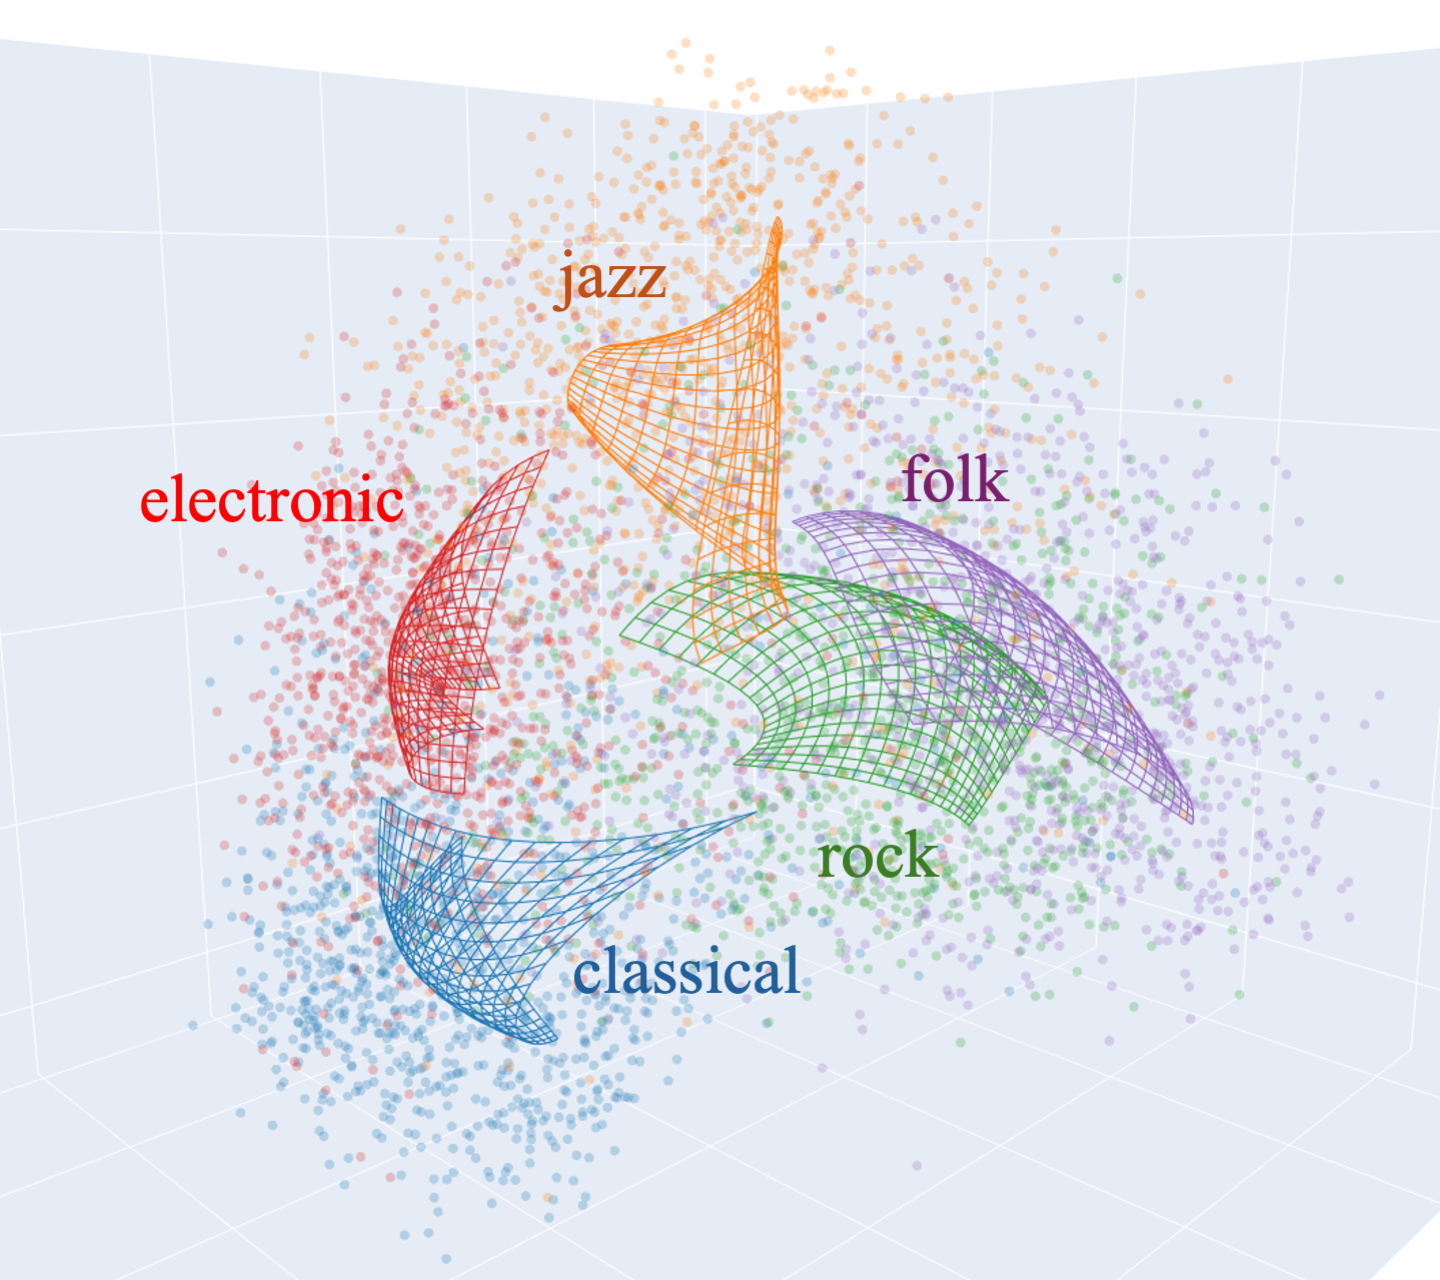
\includegraphics[width=1.0\linewidth]{fig/fig4a.png}
        \caption{Independent manifolds in $\mathcal{X}$.}
    \end{subfigure}
    \hfill
    \begin{subfigure}[t]{0.48\linewidth}
        \centering
        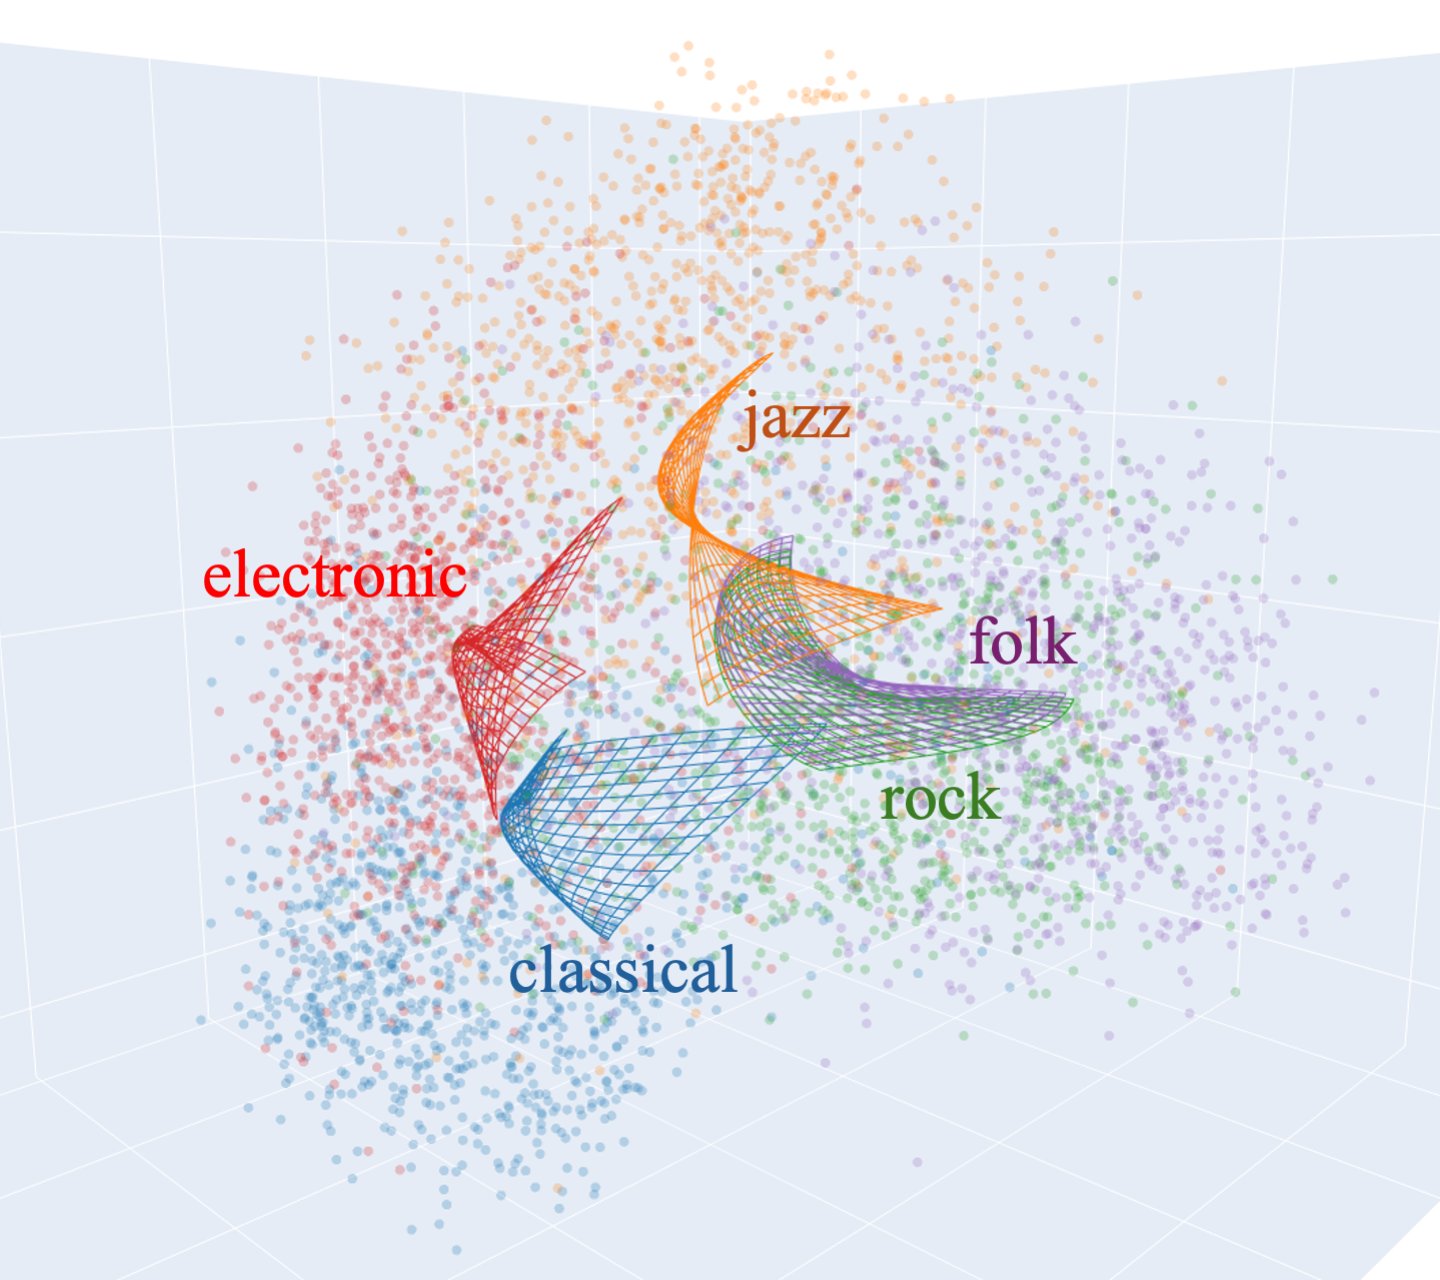
\includegraphics[width=1.0\linewidth]{fig/fig4b.png}
        \caption{The OT-FB in $\mathcal{X}$.}
    \end{subfigure}

    \vspace{2mm}

    \begin{subfigure}[t]{0.38\linewidth}
        \centering
        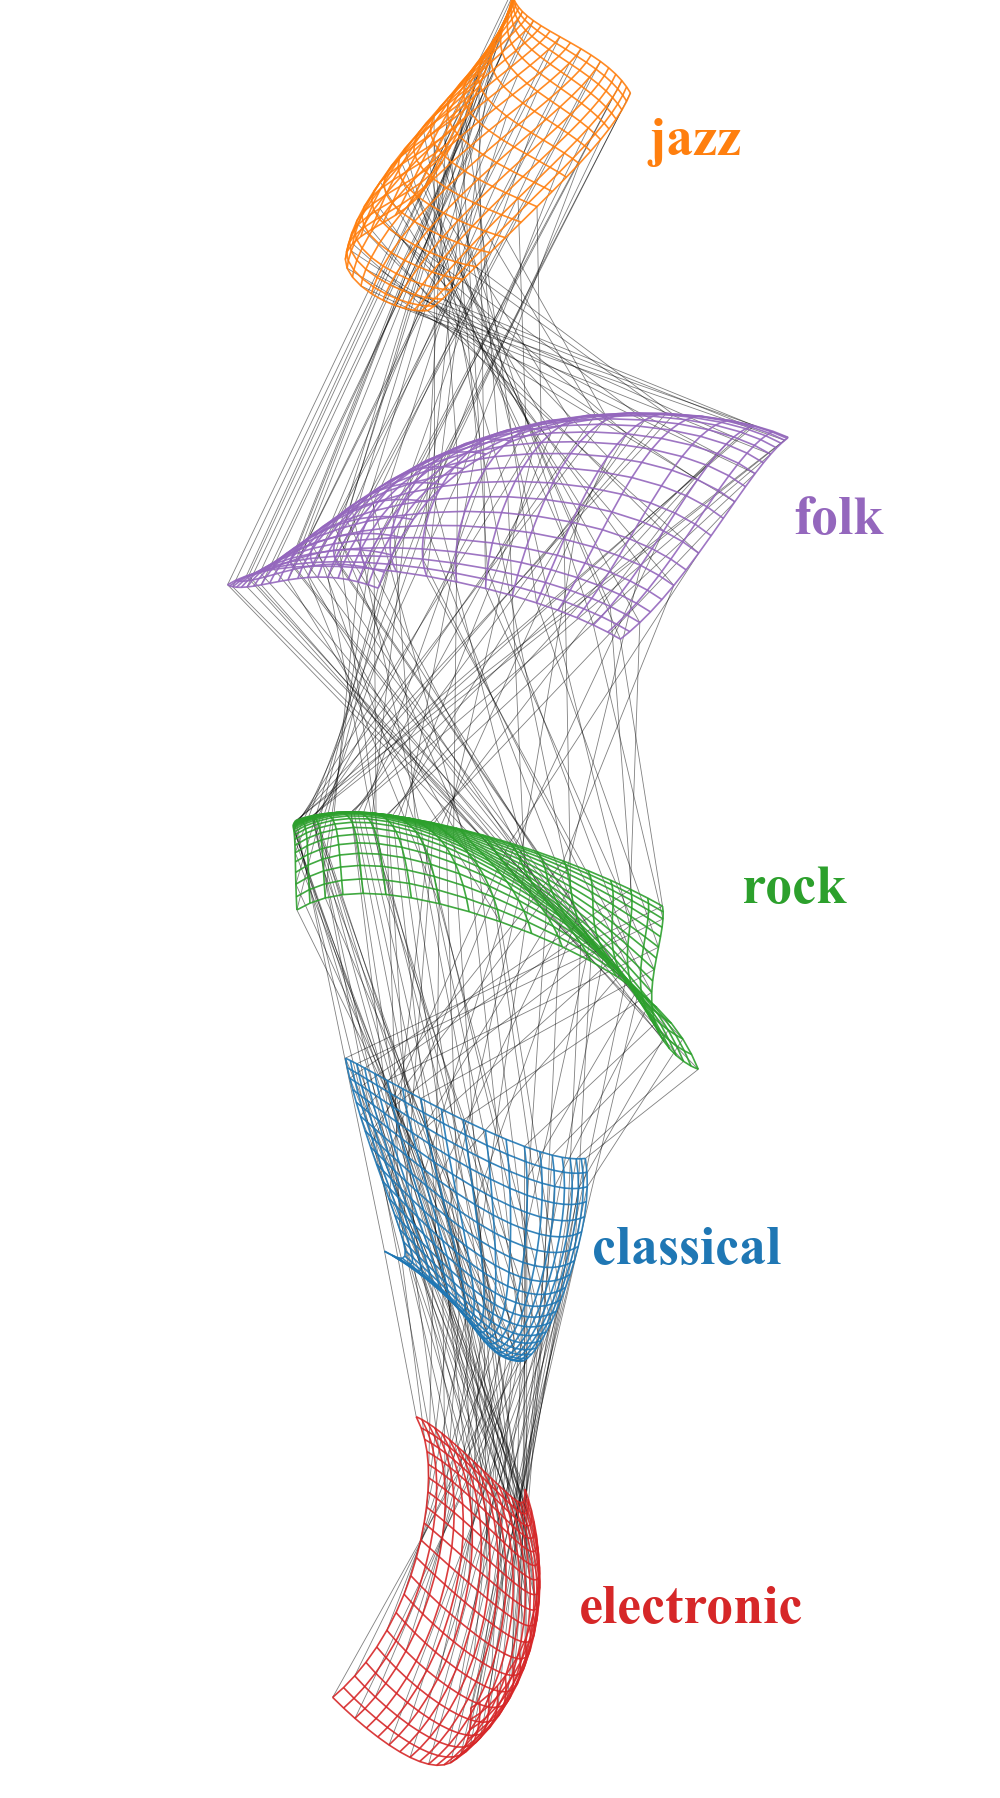
\includegraphics[width=1.0\linewidth]{fig/fig4c.png}
        \caption{Independent manifolds, stacked.}
    \end{subfigure}
    \hfill
    \begin{subfigure}[t]{0.38\linewidth}
        \centering
        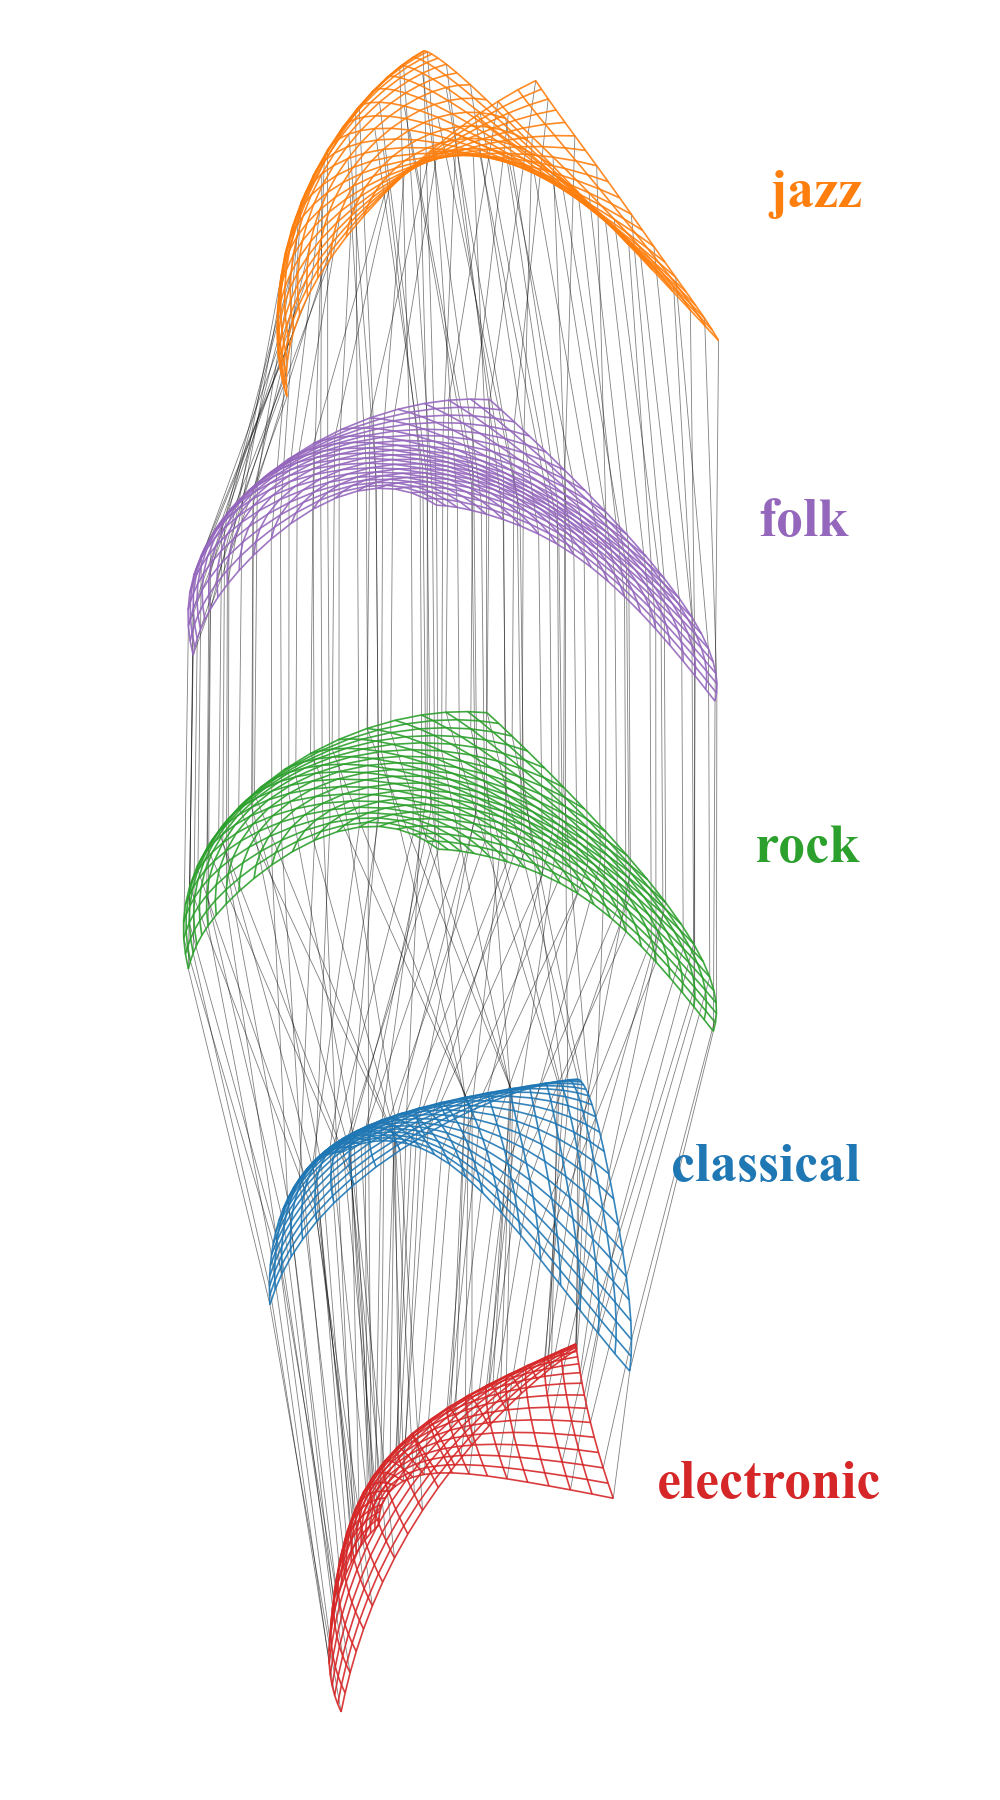
\includegraphics[width=1.0\linewidth]{fig/fig4d.png}
        \caption{The OT-FB, stacked.}
    \end{subfigure}
    \caption{
        \textbf{The five-genre OT-FB learned from MTG-Jamendo.}
        The content data (CLAP embeddings of the audio, first three
        principal components) with the genre manifolds.
        (a) Manifolds fitted independently, one per genre.
        (b) The same five learned jointly as one OT-FB.
        (c, d) The manifolds of (a) and of (b), translated apart and
        stacked as floors; each line joins the same coordinate $v$
        through all five.}
    \label{fig:mtg_otfb}
\end{figure}

%%% Subsection 5.1 %%%
\subsection{A Music Library from Sound and Genre}
\label{subsec:music_library}

\paragraph{Setup.}
The first library is built from MTG-Jamendo~\cite{Bogdanov2019}, an
openly licensed music collection. Five genres---classical, jazz, rock,
electronic, and folk---enter the library, one thousand tracks each, and
every track carries exactly one genre tag. The content data come from
sound alone: each track is embedded by CLAP~\cite{Wu2023}, a joint
audio--text encoder, over excerpts drawn from across it, then averaged,
normalized to unit norm, and reduced by PCA to ten dimensions. These
embeddings and the genre labels are all the modeling uses. The
collection also carries community tags---instruments, moods, and
themes---and they are held out, to be read afterward against the space
the sound itself has built.

\paragraph{The learned bundle.}
Figure~\ref{fig:mtg_otfb} shows the collection modeled by the OT-FB{}.
The five galaxies separate cleanly in the content space
$\mathcal{X}$: sound alone, embedded, already tells the genres apart.
In (a) a manifold is fitted to each galaxy independently; in (b) the
five are learned together as one OT-FB. The fit is much the same, but
the manifolds of (b) are floors of one bundle.

Panels (c) and (d) stack the manifolds apart as floors, each line
joining the same $v$ through all five. In (c) the lines cross and
tangle: every manifold carries a coordinate of its own. In (d) the
same lines descend in order. Five galaxies that lie apart in
$\mathcal{X}$ now share one coordinate system, and each line is a
rabbit hole: five works, one per genre, standing at the same $v$.

Both results satisfy Bias 1: in (c) as in (d), $v$ runs independently
of the genre. Bias 1 alone leaves the floors unaligned. Bias 2 aligns
them, minimizing the total length of the weft.


\begin{figure}[t]
    \centering
    \begin{minipage}[b]{0.47\textwidth}
        \centering
        \begin{subfigure}[b]{0.48\linewidth}
            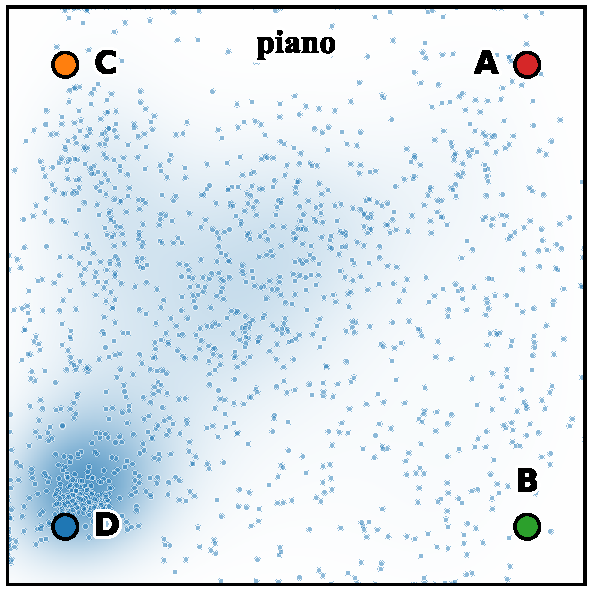
\includegraphics[width=\linewidth]{fig/fig5a.pdf}
            \caption{\textit{piano}}
        \end{subfigure}
        \hfill
        \begin{subfigure}[b]{0.48\linewidth}
            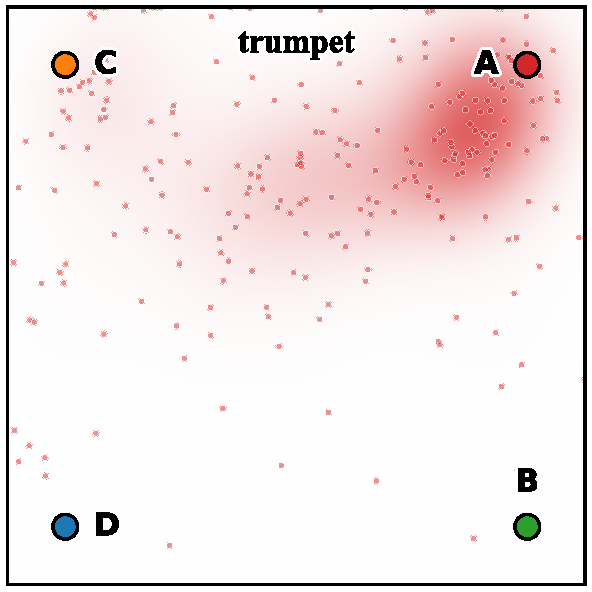
\includegraphics[width=\linewidth]{fig/fig5b.pdf}
            \caption{\textit{trumpet}}
        \end{subfigure}

        \vspace{2mm}

        \begin{subfigure}[b]{0.48\linewidth}
            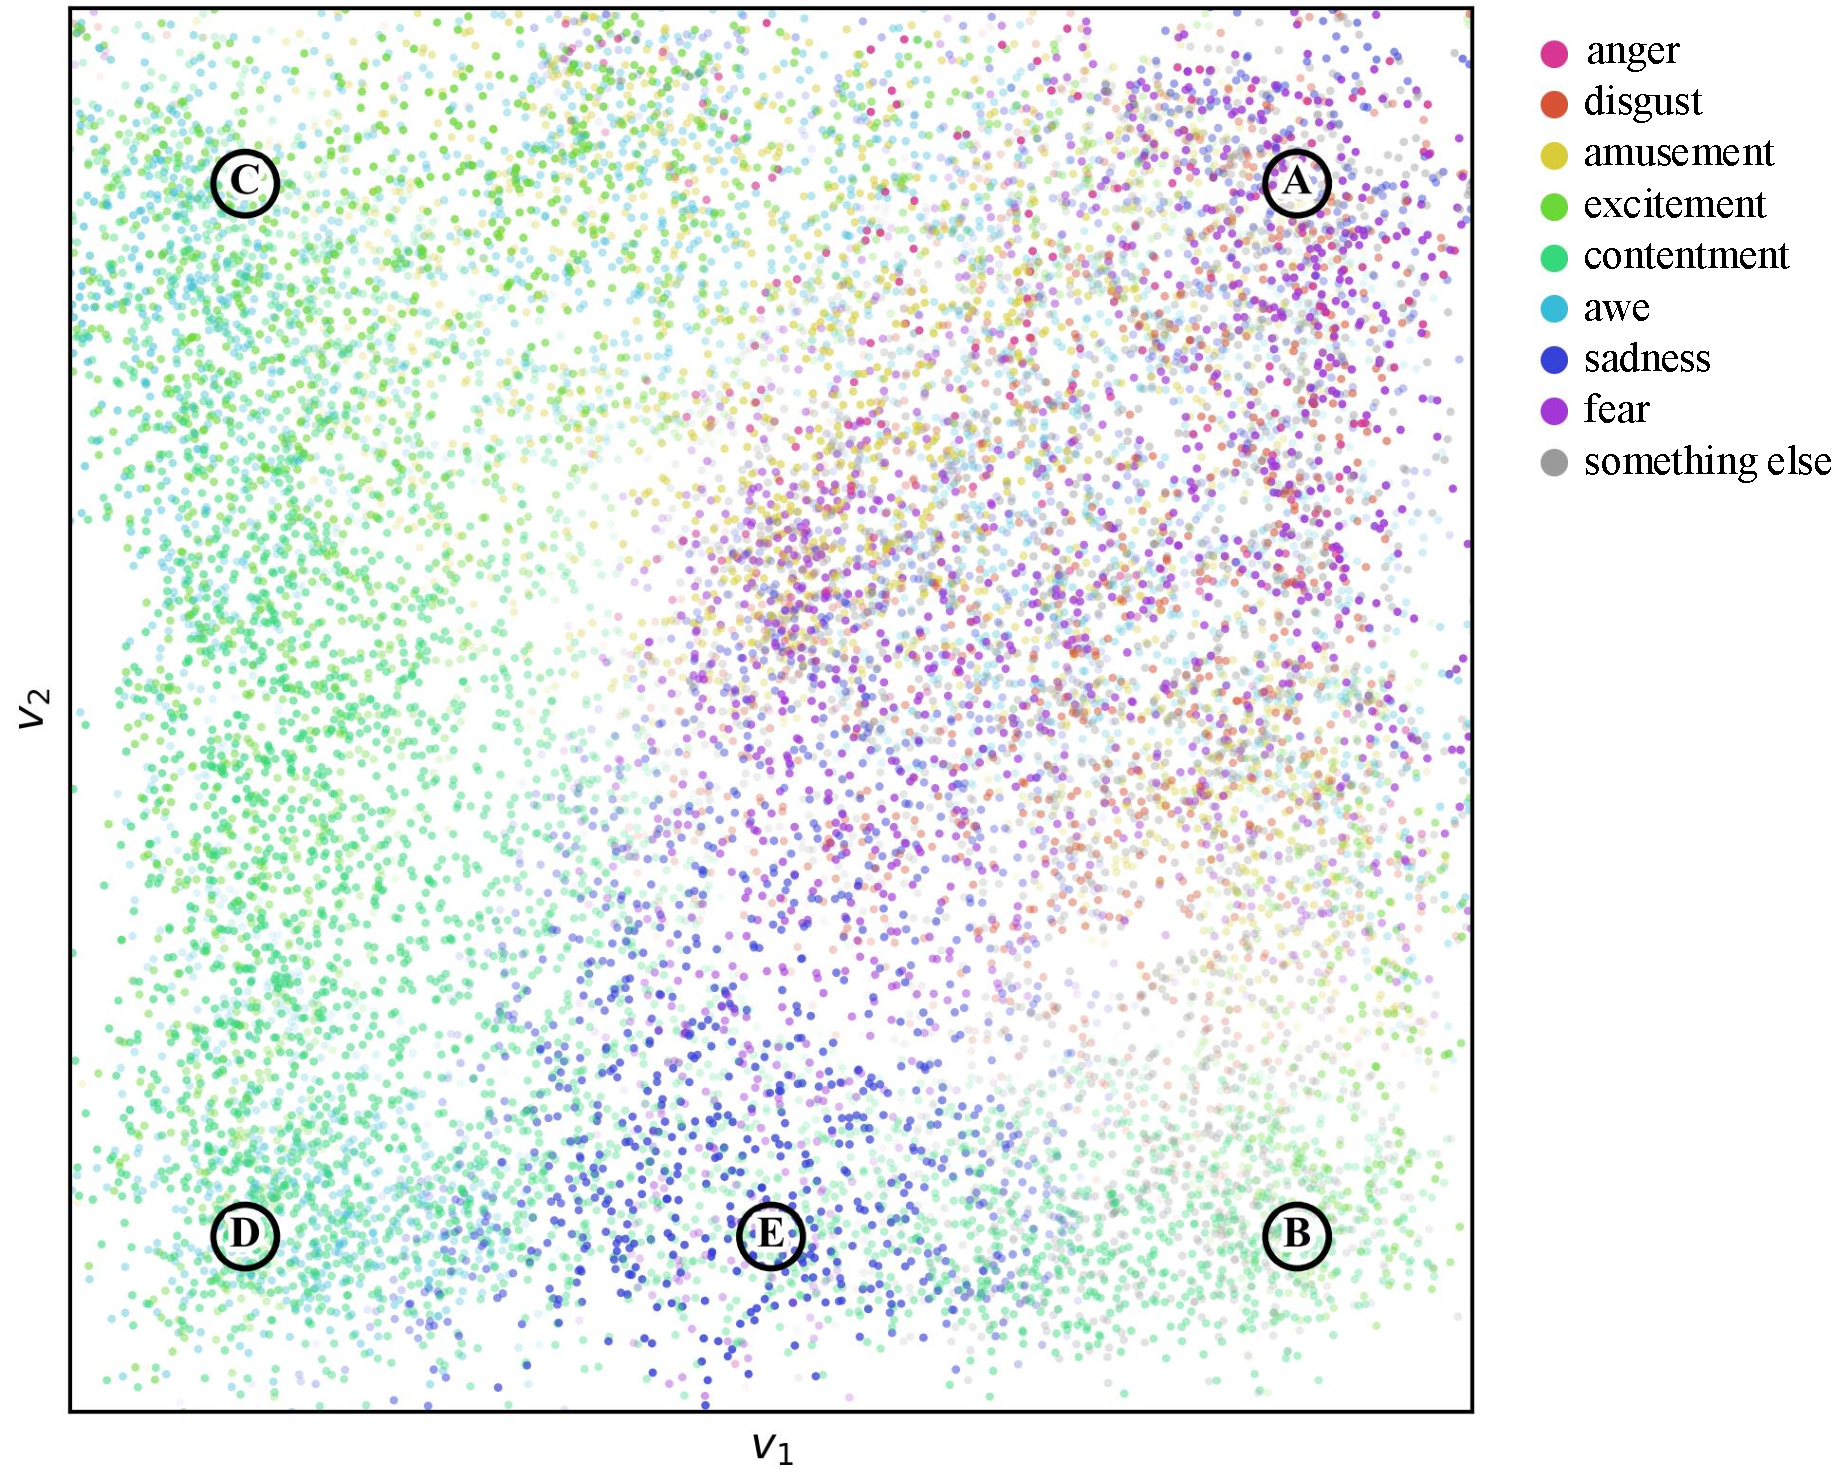
\includegraphics[width=\linewidth]{fig/fig5c.pdf}
            \caption{\textit{acoustic guitar}}
        \end{subfigure}
        \hfill
        \begin{subfigure}[b]{0.48\linewidth}
            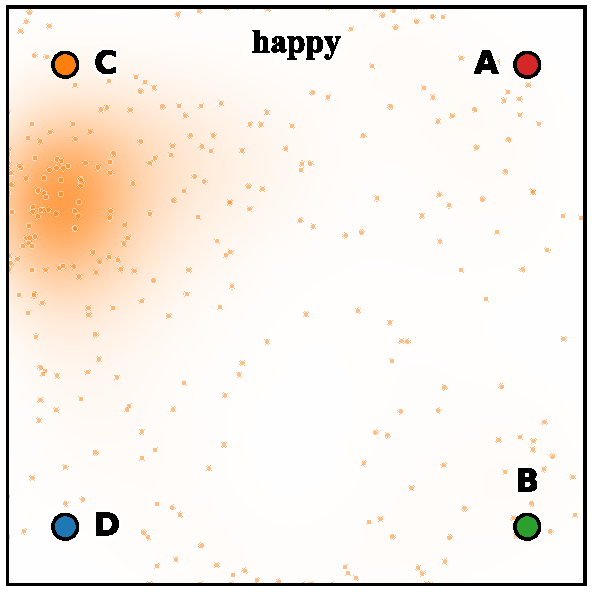
\includegraphics[width=\linewidth]{fig/fig5d.pdf}
            \caption{\textit{happy}}
        \end{subfigure}
    \end{minipage}
    \hfill
    \begin{minipage}[b]{0.51\textwidth}
        \centering
        \begin{subfigure}[b]{\linewidth}
            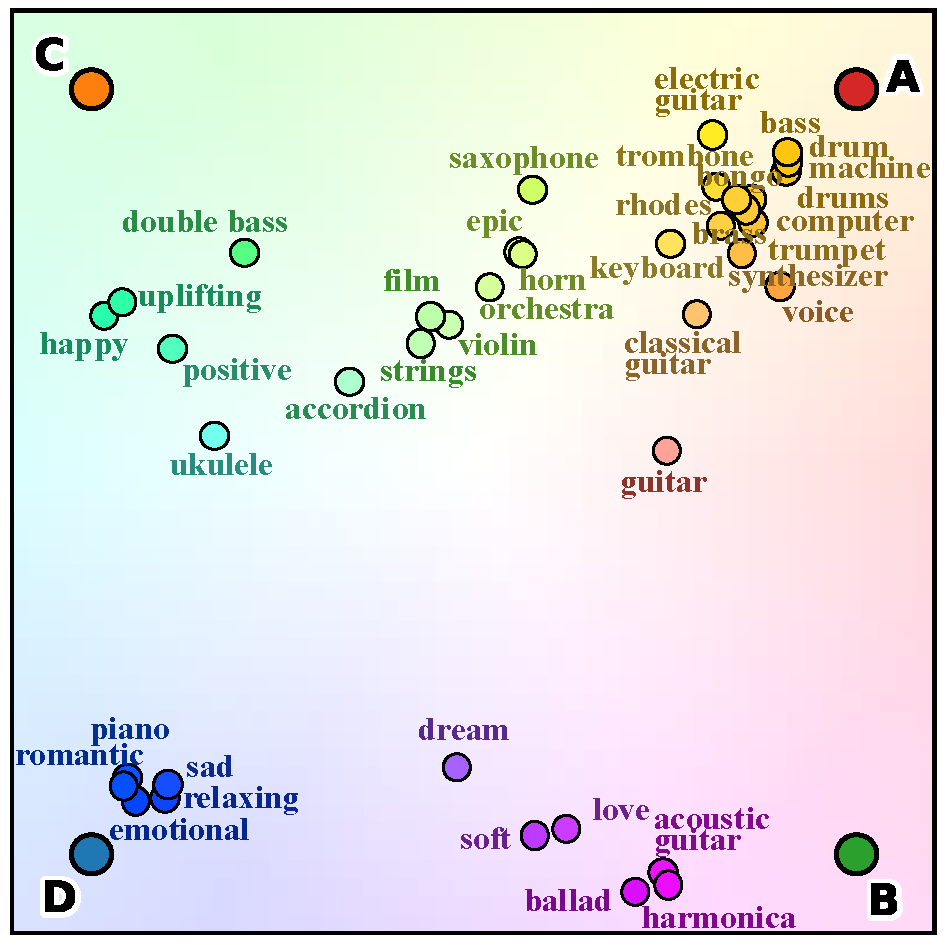
\includegraphics[width=\linewidth]{fig/fig5e.pdf}
            \caption{The landscape of $\mathcal{V}$}
        \end{subfigure}
    \end{minipage}
    \caption{
        \textbf{Reading $\mathcal{V}$ through the tags.}
        (a--d) Where four tags gather: markers show the works
        carrying the tag, and the heatmap is their density
        $p(v \mid \textit{tag})$ by kernel density estimation.
        (e) The top-40 tags by mutual information with $v$, each
        placed at the peak of its density. A peak marks where the
        works carrying the tag concentrate; the layout is not a
        clustering of the tags themselves. Points A--D are those of
        Table~\ref{tab:point_tags}.}
    \label{fig:v_tags}
\end{figure}
\begin{table}[t]
    \centering\small
    \caption{Top 20 tags by mutual information (MI) in units of
        $10^{-3}$ bit.}
    \label{tab:tag_mi}
    \begin{tabular}{@{}clc c clc@{}}
        \cmidrule[\heavyrulewidth]{1-3}
        \cmidrule[\heavyrulewidth]{5-7}
        \textbf{Rank} & \textbf{Tag}    & \textbf{MI} &  &
        \textbf{Rank} & \textbf{Tag}    & \textbf{MI}                               \\
        \cmidrule{1-3} \cmidrule{5-7}
        1             & acoustic guitar & 10.99       &  & 11 & trumpet      & 2.05 \\
        2             & piano           & 8.67        &  & 12 & saxophone    & 2.03 \\
        3             & drums           & 6.63        &  & 13 & computer     & 1.79 \\
        4             & bass            & 4.77        &  & 14 & sad          & 1.51 \\
        5             & voice           & 4.45        &  & 15 & emotional    & 1.45 \\
        6             & electric guitar & 4.11        &  & 16 & drum machine & 1.45 \\
        7             & synthesizer     & 3.60        &  & 17 & love         & 1.44 \\
        8             & ukulele         & 2.59        &  & 18 & violin       & 1.42 \\
        9             & relaxing        & 2.36        &  & 19 & romantic     & 1.41 \\
        10            & happy           & 2.17        &  & 20 & dream        & 1.38 \\
        \cmidrule[\heavyrulewidth]{1-3}
        \cmidrule[\heavyrulewidth]{5-7}
    \end{tabular}
\end{table}


\begin{table}[t]
    \centering\small
    \caption{Representative tags at the four points A--D of
        $\mathcal{V}$: the top five instrument tags and the top five
        mood/theme tags by pointwise mutual information (PMI, in bits,
        in parentheses). Negative PMI is omitted; PMI of at least 1 bit
        is in bold.}
    \label{tab:point_tags}
    \begin{tabular}{@{}c p{0.42\linewidth} p{0.42\linewidth}@{}}
        \toprule
        \textbf{Point} & \textbf{Instrument tags}                               &
        \textbf{Mood/theme tags}                                                  \\
        \midrule
        A              & \textbf{brass (1.18)}, \textbf{bongo (1.12)},
        \textbf{trombone (1.08)}, \textbf{rhodes (1.02)},
        electric guitar (0.96)
                       & fast (0.93), sport (0.84), party (0.78),
        energetic (0.32), powerful (0.30)                                         \\
        \addlinespace
        B              & \textbf{acoustic guitar (1.60)},
        \textbf{harmonica (1.57)}, \textbf{voice (1.21)},
        acousticbassguitar (0.90), percussion (0.82)
                       & \textbf{ballad (1.15)}, \textbf{love (1.04)},
        \textbf{hopeful (1.02)}, mellow (0.98), soft (0.95)                       \\
        \addlinespace
        C              & \textbf{accordion (1.63)}, \textbf{ukulele (1.41)},
        \textbf{double bass (1.29)}, \textbf{trombone (1.15)},
        \textbf{saxophone (1.10)}
                       & \textbf{funny (1.64)}, commercial (0.94), sexy (0.91),
        retro (0.89), summer (0.88)                                               \\
        \addlinespace
        D              & \textbf{piano (1.68)}, pad (0.47)
                       & \textbf{relaxing (1.97)}, \textbf{romantic (1.97)},
        \textbf{sad (1.78)}, \textbf{emotional (1.62)},
        \textbf{calm (1.57)}                                                      \\
        \bottomrule
    \end{tabular}
\end{table}

\paragraph{Reading $\mathcal{V}$ through the tags.} What does the facet-induced
connotation space $\mathcal{V}$ hold? The tags held out of the
modeling---instruments, moods, and themes---give the reading. Each tag defines a
density over $\mathcal{V}$: the distribution $p(v \mid \textit{tag})$ of the
works that carry it. Figure~\ref{fig:v_tags}(a--d) shows four of
them---\textit{piano}, \textit{trumpet}, \textit{acoustic guitar}, and
\textit{happy}. Each peaks at a place of its own, yet the four densities
overlap---connotation runs as a continuous spectrum, not as discrete regions.

Tags differ in how much they tell about $v$. The mutual information
$\mathrm{MI}[v; \textit{tag}]$ measures it: how unevenly the works
carrying the tag fall over $\mathcal{V}$. Table~\ref{tab:tag_mi}
lists the top twenty. Instruments occupy the upper ranks, and moods
follow.

\paragraph{The landscape of $\mathcal{V}$.}
Figure~\ref{fig:v_tags}(e) widens the reading to the top forty tags,
each placed at the peak of its density $p(v \mid \textit{tag})$. Each
tag still spreads around its peak, as (a--d) show; the map marks
where it gathers most.

The landscape divides in two. The upper half is lively: to the right,
drums, bass, electric guitar, and brass---powerful music; to the
left, happy and uplifting. The lower half is quiet: to the right,
acoustic guitar, with love and dream---ballads; to the left, piano,
with emotional, relaxing, sad, and romantic. The two coordinates of
$\mathcal{V}$ carry no names, no more than a principal component
does; yet the landscape they span is legible from end to end.

Table~\ref{tab:point_tags} reads four points more closely: the
corners A--D, each a rabbit hole, seen through the tags concentrated
there. At A the music is fast and energetic, played by brass and
bongo; at B, love ballads on acoustic guitar; at C, funny songs on
accordion and ukulele; at D, piano, relaxing and sad. No single tag
names a point; the tags gathered there do.

\paragraph{What $\mathcal{V}$ represents.}
The tags have read $\mathcal{V}$ as a continuous spectrum. Connotation
itself, though, is known by hearing rather than by words. It lies in
what the works gathered at one point have in common, and no single
word holds it. The tags cannot name it; they let the seeker guess what
a point holds, and a guess is enough to start walking.

What $\mathcal{V}$ holds follows from the facet. Genre was the only
facet, so all else---instruments, moods, themes---was left to
connotation. Which of them, then, does $\mathcal{V}$ carry?

$\mathcal{V}$ carries the two as one. An instrument tends to bring its
own moods---the ring of brass, the cheer of a ukulele, the warmth of
an acoustic guitar. So tags do not settle at points of $\mathcal{V}$.
Each one spreads over a stretch of the spectrum, and the stretches
overlap: \textit{piano} peaks at the lower left, among relaxing and
sad, and reaches the upper right as well, where the music runs
energetic (Figure~\ref{fig:v_tags}(a)). $\mathcal{V}$ is a qualia
spectrum, and its qualia are instrument and mood joined.
\textit{Principal} means this: the two dimensions that account for
that joining with least error (Section~\ref{subsec:content_space}).

A single point of $\mathcal{V}$ does not hold a single kind of music.
The works gathered there are alike in connotation, yet they run from
genre to genre; the space is one, shared by the five. Each point is a
rabbit hole, opening at the same $v$ on every floor. At point A, rock
is energetic music driven by drums; through the hole, on the classical
floor, brass plays with the same force.

Return now to the visitor of Section~\ref{sec:introduction}. The
catalogue told him \textit{trumpet}, and most trumpet music sits at A,
fast and played with force. That is the crowd of trumpeters his search
returned, and almost none of it was what he wanted. What he wanted
lies at D, where trumpets are few, yet present
(Figure~\ref{fig:v_tags}(b)). The name Miles Davis carries him to the
jazz floor and to D upon it, and the hole at D opens onto the
emotional pianos of every other floor. In
Section~\ref{sec:introduction} he made that passage by chance, weeks
later, in a train station. Here it lies under his feet.


\begin{figure}[p]
    \centering
    \begin{subfigure}[b]{0.45\linewidth}
        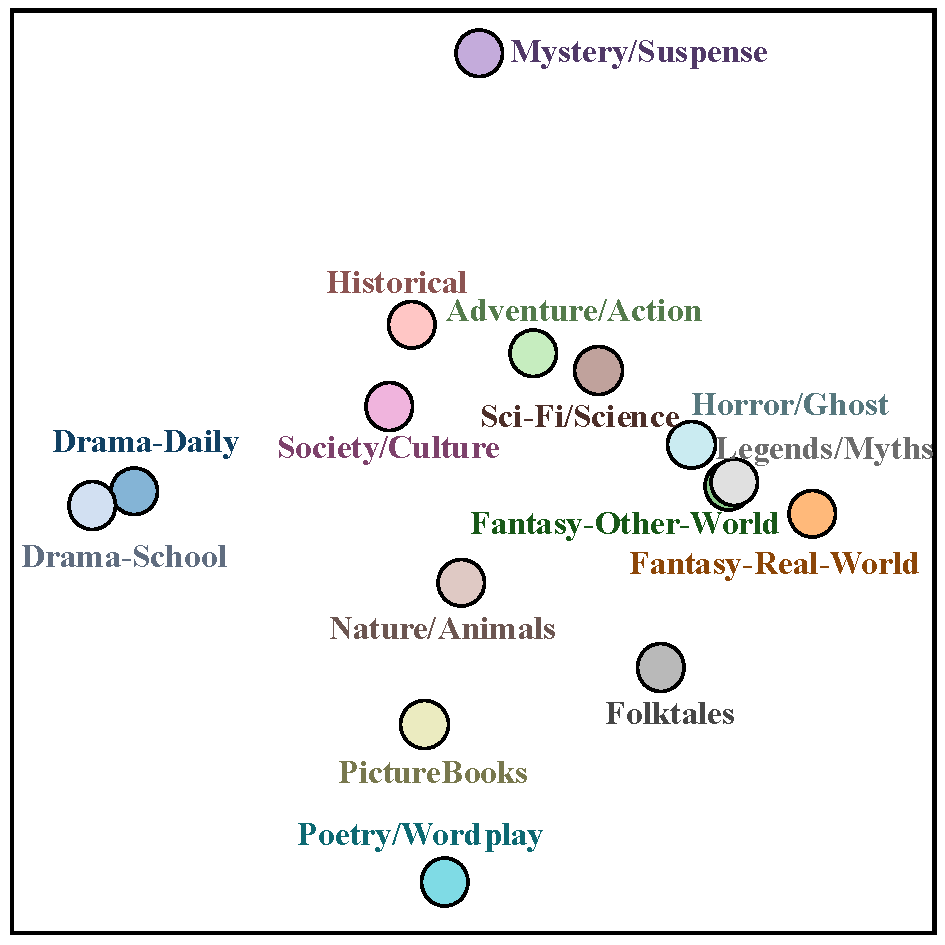
\includegraphics[width=\linewidth]{fig/fig6a.pdf}
        \caption{Spectrum of style/subject}
    \end{subfigure}
    \hfill
    \begin{subfigure}[b]{0.45\linewidth}
        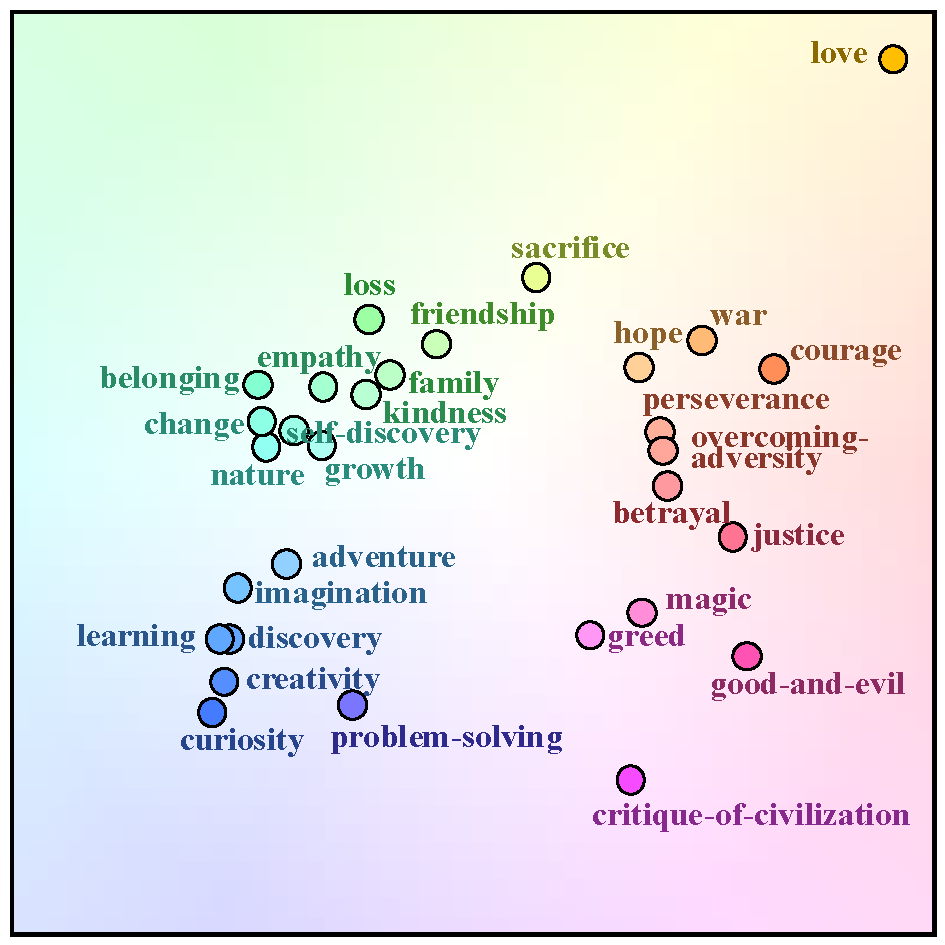
\includegraphics[width=\linewidth]{fig/fig6b.pdf}
        \caption{$\mathcal{U}$ for style/subject}
    \end{subfigure}

    \vspace{2mm}

    \begin{subfigure}[b]{0.42\linewidth}
        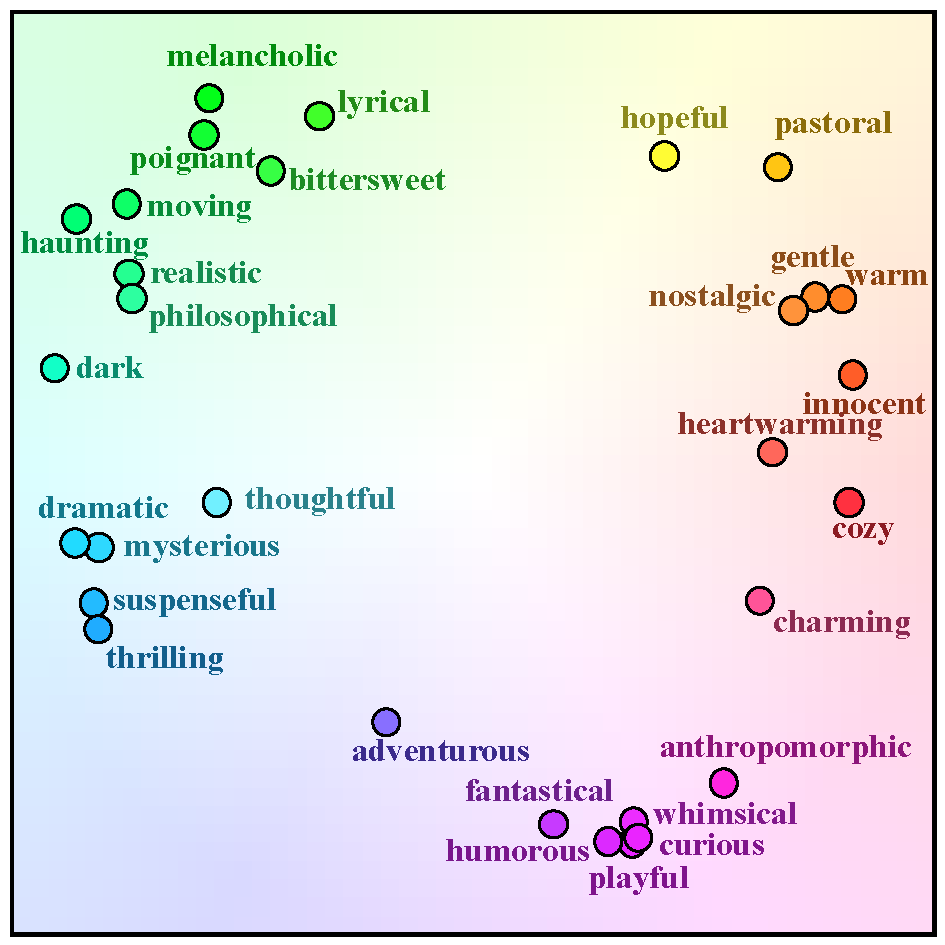
\includegraphics[width=\linewidth]{fig/fig6c.pdf}
        \caption{Words on $\mathcal{V}$}
    \end{subfigure}
    \hfill
    \begin{subfigure}[b]{0.55\linewidth}
        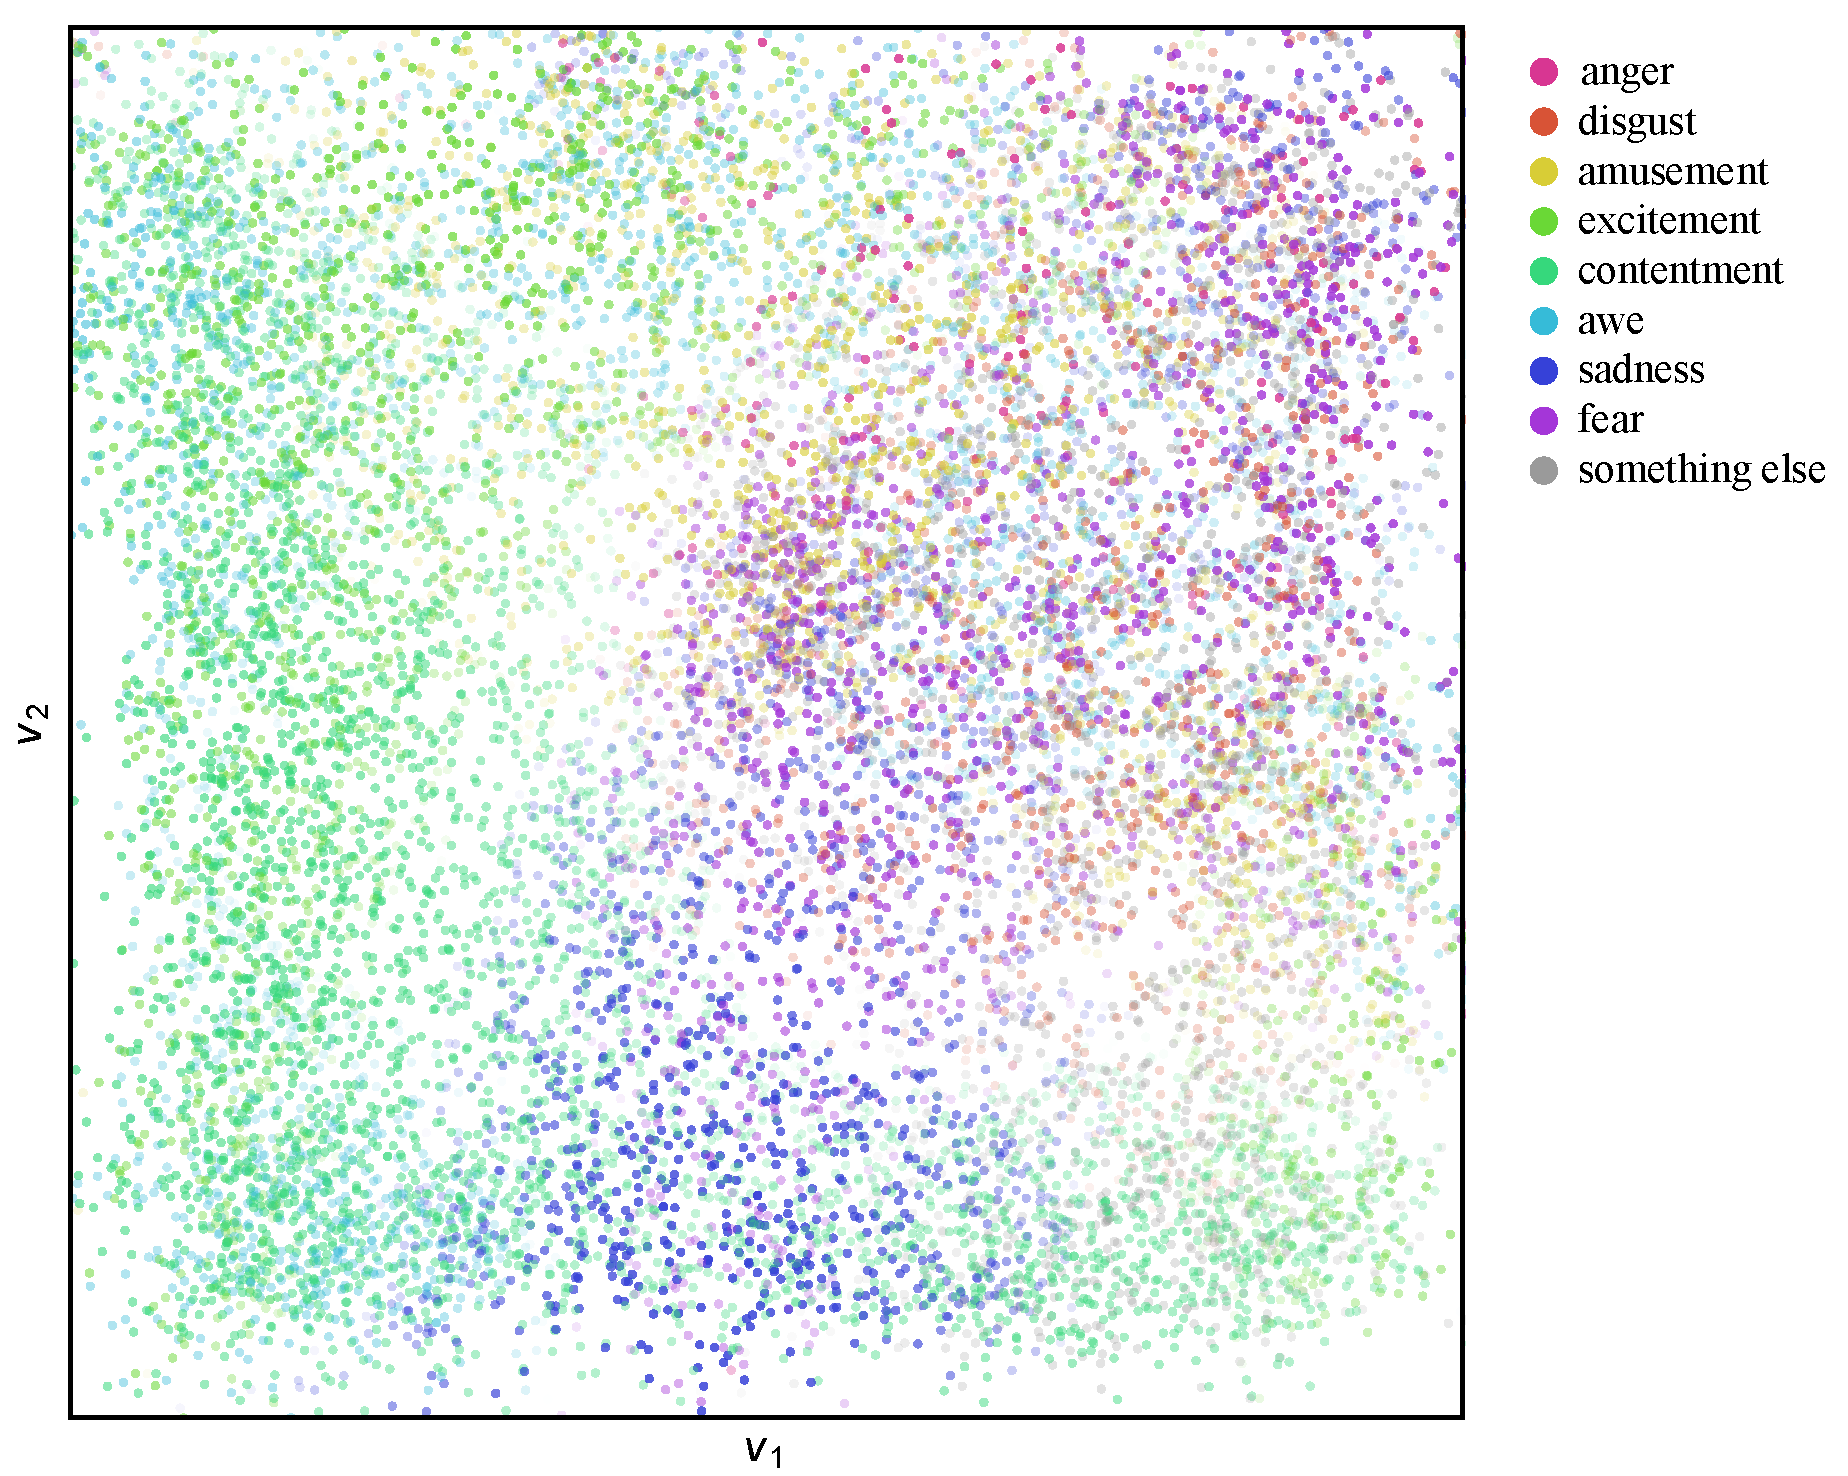
\includegraphics[width=\linewidth]{fig/fig6d.pdf}
        \caption{Emotion on $\mathcal{V}$}
    \end{subfigure}
    \caption{
        \textbf{The twenty-six-floor OT-FB learned from WikiArt.}
        (a) The manifolds in the content space $\mathcal{X}$ (CLIP
        embeddings of the images, first three principal components), one
        per floor.
        (b) The denotation space $\mathcal{U}$. Each marker is one floor,
        its shape the subject: $\triangle$ landscape, $\square$ genre
        painting, $\Diamond$ religious painting, $\bigcirc$ portrait.
        Style runs across, subject runs down.
        (c, d) The connotation space $\mathcal{V}$, read through the
        held-out ArtEmis annotations. Markers sit at the peak of each
        density $p(v \mid \cdot)$: in (c) pairs of emotions, since a
        single emotion peaks in several places while a pair settles in
        one; in (d) words. Larger markers and labels carry higher
        pointwise mutual information with $v$, on each panel's own scale.
        Both panels share one background, the emotion spectrum: the nine
        emotion densities are turned into PPMI, reduced to three axes by
        SVD, and printed as cyan, magenta, and yellow ink on white. Hue
        tells which emotions gather; lightness tells how strongly. White
        marks where no emotion stands out.}
    \label{fig:wikiart}
\end{figure}

%%% Subsection 5.2 %%%
\subsection{A Painting Library from Image, Style, and Subject}

\paragraph{Setup.}
The second library is built from WikiArt, a community-curated
encyclopedia of visual art. Here two facets are given at once: style
and subject. Nine styles, from Baroque to Cubism, meet six subjects
such as landscape and portrait, and every painting carries one name
from each: \textit{Impressionism--landscape}, for instance. All
fifty-four combinations are filled, with up to two hundred paintings
each and nearly nine thousand in all; Figure~\ref{fig:wikiart}(b)
names them. The content data come from the image alone: each painting
is resized whole to 224 by 224, never cropped, and embedded by
CLIP~\citep{Radford2021,Cherti2023}, a joint image--text encoder, then
normalized to unit norm, centered, and reduced by PCA to ten
dimensions. These embeddings and the two labels are all the modeling
uses. The collection also carries ArtEmis~\citep{Achlioptas2021}---%
nine emotions, chosen by a median of six viewers per painting---and
these are held out, as the community tags were.

\paragraph{The learned bundle.}
Figure~\ref{fig:wikiart}(a) shows the fifty-four manifolds in
$\mathcal{X}$, laid out by style and subject. Colour marks $v$: one
colour, one connotation, on every manifold alike. From cell to cell
the surfaces bend and stretch, yet the colours hold their places.
Fifty-four manifolds make one spectrum, as the five genres did.

Read as a library, each style is a floor, and each floor holds six
rooms, one per subject. The rabbit holes join every room to every
other. A visitor may leap to another subject on the same floor, or to
the same subject on another floor, or take both leaps at once---from a
Baroque portrait to a Cubist landscape, in one step. Every leap moves
$u$ and leaves $v$ where it was: the connotation is kept.


\begin{table}[t]
    \centering\small
    \caption{Representative tags at the four points A--D of
        $\mathcal{V}$: the top five annotated words, annotated
        emotions, and painting features by pointwise mutual
        information (PMI, in bits, in parentheses). Negative PMI
        is omitted; PMI of at least 1 bit is in bold. Painting
        features are binarised within each of the 54 classes at
        the 20\% tails, so they are independent of both
        CLIP and the annotations.}
    \label{tab:point_tags_wikiart}
    \begin{tabular}{@{}c p{0.25\linewidth} p{0.24\linewidth} p{0.35\linewidth}@{}}
        \toprule
        \textbf{Point}              & \textbf{Annotated words}                                                                    &
        \textbf{Annotated emotions} & \textbf{Painting features}                                                                                                                                                                                                                                                                                                \\
        \midrule
        A                           & \textbf{black (1.13)}, \textbf{lines (1.10)}, simple (0.87), men (0.84), white (0.78)       & anger (0.67), fear (0.65), disgust (0.26), sadness (0.22), something else (0.19) & \textbf{chroma range (lo) (1.18)}, \textbf{colorfulness (lo) (1.14)}, hue variety (lo) (0.94), chroma (lo) (0.93), lightness (hi) (0.79) \\
        \addlinespace
        B                           & \textbf{flowers (1.08)}, fruit (0.69), red (0.66), colorful (0.62), pink (0.61)             & contentment (0.18), something else (0.13), excitement (0.13), disgust (0.05)     & coarseness (lo) (0.50), colorfulness (hi) (0.50), lightness range (lo) (0.44), chroma (hi) (0.41), hue variety (hi) (0.40)               \\
        \addlinespace
        C                           & \textbf{women (1.11)}, \textbf{people (1.02)}, field (0.99), animals (0.89), vibrant (0.81) & excitement (0.36), awe (0.16), contentment (0.09)                                & self-similarity (hi) (0.94), edge strength (hi) (0.91), brushwork energy (hi) (0.87), anisotropy (lo) (0.85), coarseness (lo) (0.75)     \\
        \addlinespace
        D                           & \textbf{dress (1.23)}, fruit (0.88), street (0.87), skin (0.65), city (0.64)                & contentment (0.27), awe (0.13), excitement (0.07)                                & energy height (hi) (0.59), energy spread (lo) (0.53), lightness range (hi) (0.48), center focus (hi) (0.48), warm (hi) (0.47)            \\
        \bottomrule
    \end{tabular}
\end{table}


\paragraph{The facet map.}
Figure~\ref{fig:wikiart}(b) shows the denotation space $\mathcal{U}$:
the floor-room arrangement of the library. Two facets went in as two
axes, and each axis returned an order.

Style runs in the order of its dates, Baroque to Cubism, though no
date entered the modeling. The spacing is uneven: Expressionism and
Fauvism nearly touch, because their paintings nearly touch in
$\mathcal{X}$.

Subject runs from far to near---cityscape and landscape, then still
life, then genre painting and portrait, and last nude painting. The
view moves from the distant scene to the human body.

Nobody set these orders. Transport places each focus where its works
ask it to stand.

\paragraph{Reading $\mathcal{V}$.}
Figures~\ref{fig:wikiart}(c) and (d) read $\mathcal{V}$ as the tags
read it before. The held-out ArtEmis annotations give two readings:
the emotions viewers reported, and the words they wrote, each placed
at the peak of its density. The background of both panels is the
emotion spectrum itself, so the two readings lie one upon the other.

The reading runs as it did for music. Neither emotions nor words
settle at points; each spreads over a stretch of the spectrum, and the
stretches overlap. And again the two are joined. Where fear gathers,
at the upper left, the words are \textit{dark}, \textit{black},
\textit{lines}, \textit{figure}. Where awe gathers, at the upper
right, they are \textit{mountains}, \textit{hills}, \textit{clouds},
\textit{blue}. Where contentment gathers, below, they are
\textit{flowers}, \textit{dress}, \textit{young}, \textit{peaceful}.
Here too $\mathcal{V}$ is a qualia spectrum, and its qualia are
subject and feeling joined.